%% LaTeX2e class for student theses
%% sections/content.tex
%% 
%% Karlsruhe Institute of Technology
%% Institute for Program Structures and Data Organization
%% Chair for Software Design and Quality (SDQ)
%%
%% Dr.-Ing. Erik Burger
%% burger@kit.edu
%%
%% Version 1.3, 2016-12-29

\chapter{iObserve Extension}
\label{ch:iObserve}

iObserve was briefly introduced in \autoref{sec:Foundations:iobserve}. iObserve uses Kieker (\autoref{sec:Foundations:Kieker}) to gain real-time information about an observed (distributed) software system. iObserve transforms these information onto a Palladio Component Model. This model is referenced as \textit{runtime PCM} or \textit{runtime model}, since it reflects the actual observed software system during runtime \cite{Heinrich.2016}.


\section{Kieker}
\label{sec:Kieker:privacy}

\textit{Kieker} was also briefly introduced in foundational work (see \autoref{sec:Foundations:Kieker}). Kieker had already specified the geo-location record for transporting the geo-location information form the observed system to Kieker. However, a probe was still missing. As a result, we created a heart-beat/periodic probe (\textit{ServerGeoLocationSampler}). This probe uses a \textit{ICountryInvestigator} to determine the actual geo-location and creates a \textit{ServerGeoLocation} record (see \autoref{fig:geoLocationRecord}).

As an alternative, we could have created an event-based geo-location probe. Possible event could have been the component deployment or un-deployment or the server acquiring or release. This however, would mean, there wouldn't be a geo-location update between these events and potential privacy violation could stay undetected indefinitely or for a long period. Even though a heart-beat probe often takes longer to send an initial record, eventual changes will definitely be detected due to the regular updates.

\begin{figure}[h]
	\centering
	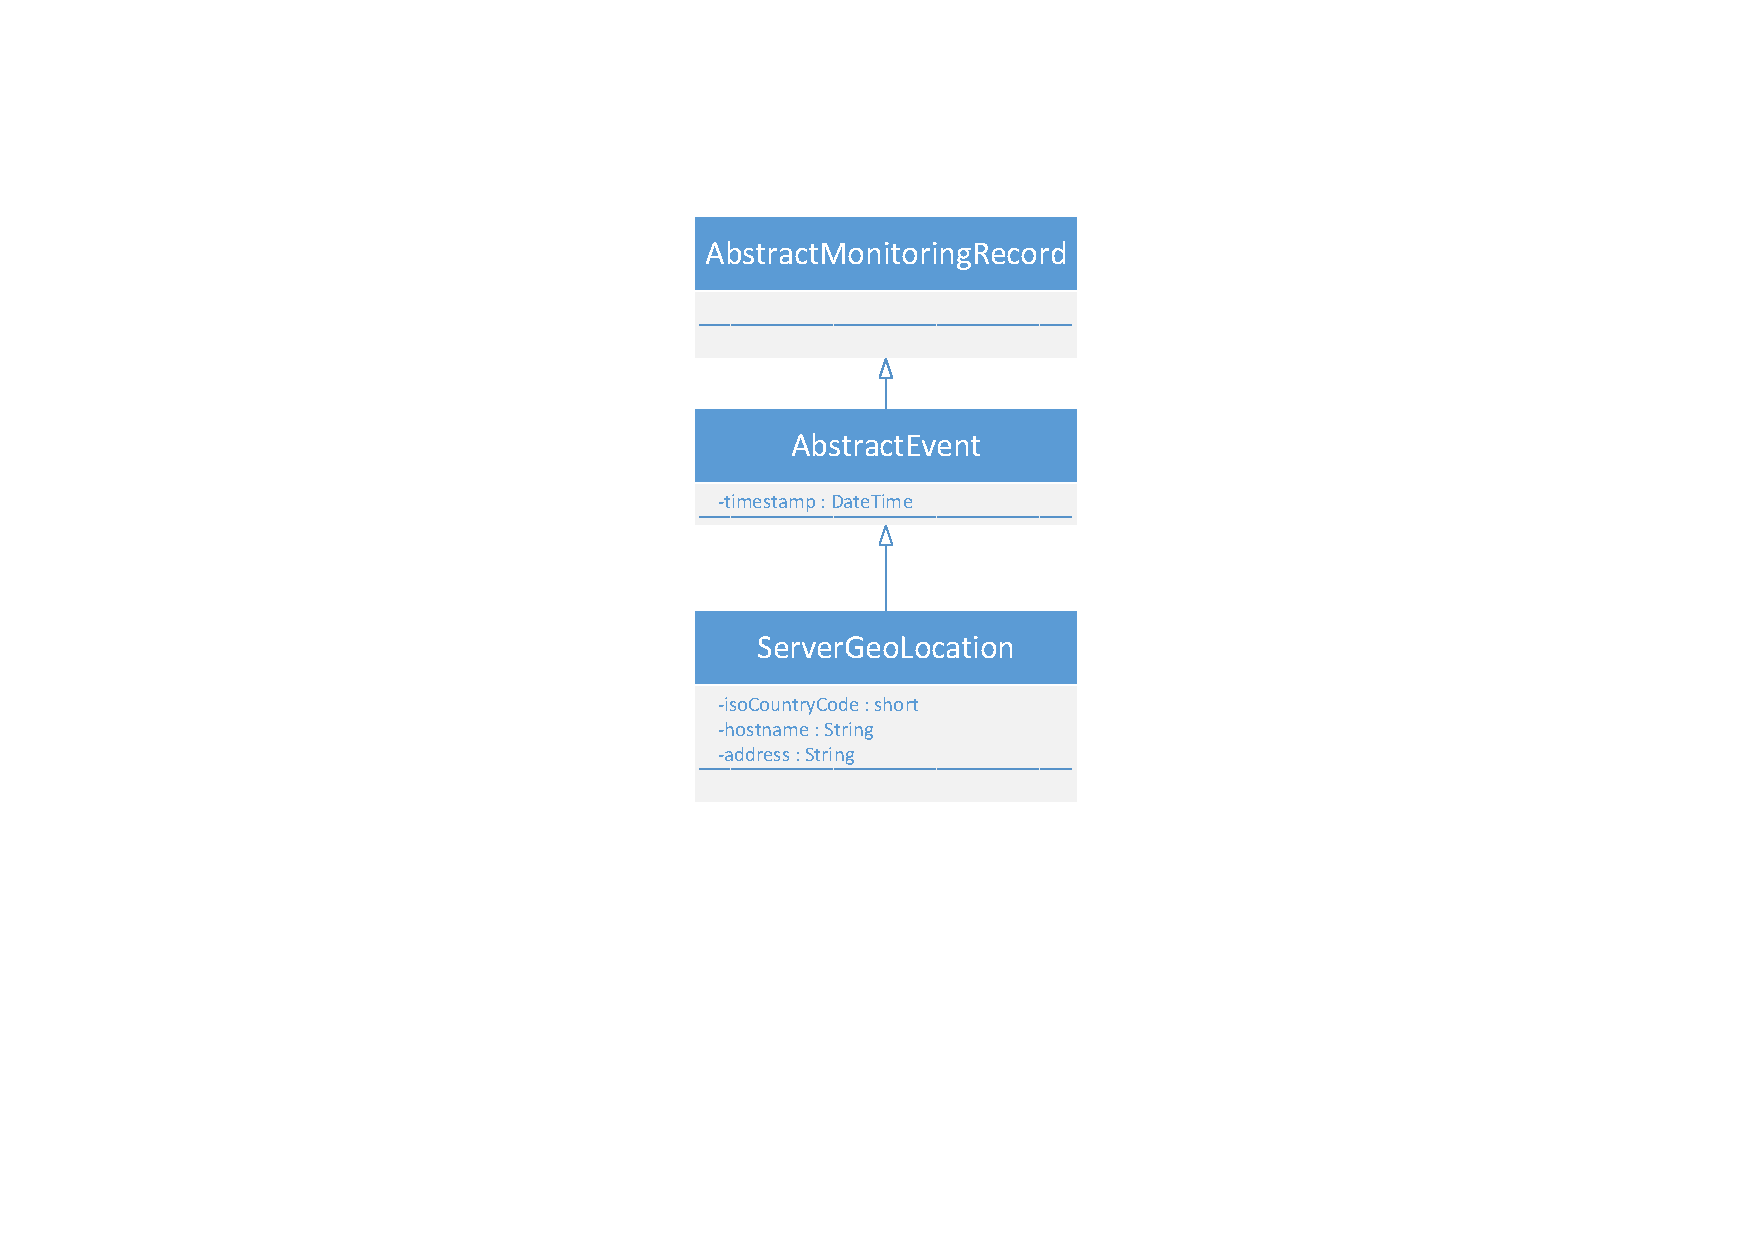
\includegraphics[trim = 10mm 70mm 5mm 5mm, clip, width=1.00\textwidth]{graphs/GeoLocationRecord}
	\caption{Server Geo-Location Record and Sampler}
	\label{fig:geoLocationRecord}
\end{figure}

Kieker gather the information from the observed system probes and redirects them to iObserve. More information on Kieker can be found at \cite{kieker.web}.

\section{iObserve Privacy}
\label{sec:iObserve:privacy}
%Kieker => Map onto PCM (Transformation)

iObserve uses the teetime framework. Its allows easy pipeline building by connecting matching input and output ports during runtime \cite{teetime.16.05.2017}. This mechanism is used by iObserve to invoke different transformations. Based on the received \textit{Monitoring Record}, the according output port gets invoked and the matching transformation will be executed.

%Geo-location transformation
For the \textit{ServerGeoLocation Record} (see \autoref{fig:geoLocationRecord}) another output port and transformation was added. The transformation uses the records host and address field to find the record sending resource container. The according geo-location attribute of the \textit{Resource Container Privacy} is compared to the incoming geo-location and updated if needed.

%Extend Framework
\begin{figure}[h]
	\centering
	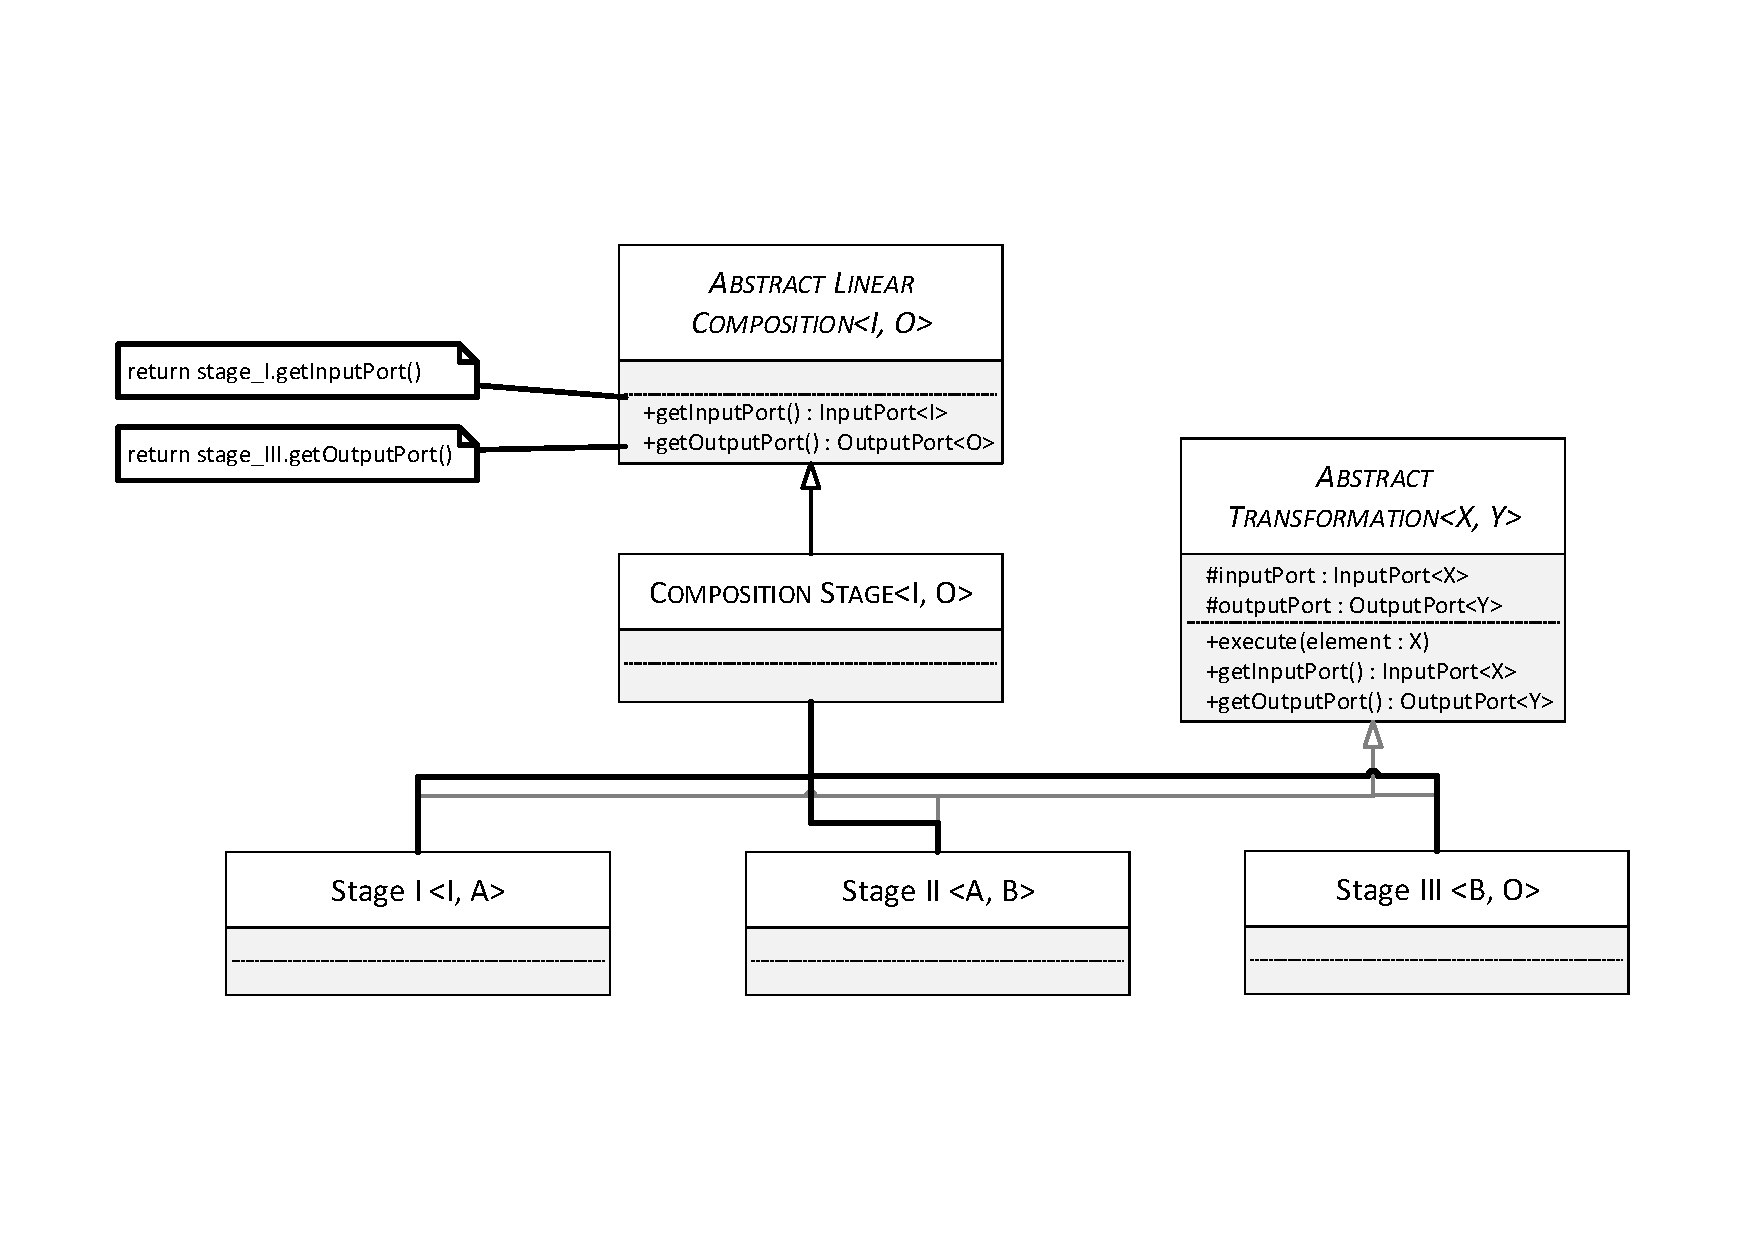
\includegraphics[trim = 20mm 40mm 20mm 35mm, clip, width=0.85\textwidth]{graphs/StageComposition}
	\caption{iObserve Privacy Filter}
	\label{fig:filterstage}
\end{figure}

iObserve has a well defined structure due to the teetime framework. We decided to keep this structure and extend it. \autoref{fig:pipeline} shows the conceptual filter pipeline structure for our planned extension. One conceptual stage usually consists if several sub tasks. The system adaptation, for example, consists of an adaptation calculation, an adaptation calculation and an execution. To embrace re-usability and lose coupling, we decided to keep on using the teetime framework structure and compose one conceptual stage out of several sub-stages. \autoref{fig:filterstage} shows the general structure of a conceptual stage. The \textit{Composistion Stage} functions as a wrapper for the conceptual filter, while the \textit{Stages} I to III represent the sub-tasks.

This structure does not only allow easy restructuring of the conceptual pipeline and encapsulates the sub-tasks, it also allows for simple reuse and a clear separation of concerns. 
For the teetime framework, the filter stages looks like a series of linear connected stages, while the developer gets easy to handle packages. It is worth mentioning, that Stages linked to each other require matching data. The actual task executed, must be placed inside the \textit{execute} method.

The extended iObserve contains the following conceptual filter stages: \textit{Monitoring}, \textit{Snapshot} (creates a copy of the current runtime model), \textit{Privacy Analysis}, \textit{Model Generation}, \textit{System Adaptation} and \textit{Evaluation}. In the remainder of this thesis the extended iObserve is referenced as \textit{iObserve Privacy}, so potential misunderstandings are avoided.



